%!TEX root = ../PP.tex


\chapter{Einführung}\label{einleitung}

Die Bachelorarbeit setzt das vorangegangene Praxisprojekt mit dem Thema „Konzeption eines erweiterten Buches als Tonträger zur Verknüpfung von Audio und Interaktion zur Aufwertung kreativer Audiowerke“ fort.

\section{Das digitale Klangbuch}
Der Umgang mit und die Wertschätzung von Musik\footnote{Musik: Im Sinne von reproduzierbarer Musik auf Tonträgern u. Ä.} hat sich seit der Schallplatte bis zur heutigen Zeit stark verändert.\\

{\centering\textcolor{m_pink}{\textit{"Musik wird nicht mehr wertgeschätzt."}}\\\hfill\begin{tiny}{Klaus Warstat \cite{K01}}\end{tiny}}\\

Musik ist heutzutage ein allgegenwärtiges Konsumgut, das weniger wertgeschätzt wird und die Bereitschaft für Musik zu zahlen ist stark gesunken.\cite{Spotify} Dieser Trend wird von Musikern, Künstlern und Musikfans als Verlust empfunden.\cite{K01}\cite{Lost}\\


Eine Idee, um diesem Trend etwas entgegen zu setzen, ist das Schaffen eines neuen Mediums - das digitale Klangbuch. Das Konzept des digitalen Klangbuchs sieht ein großformatiges, physisches Buch als erweitertes, interaktives \gls{artwork} und sinnliches Gesamtpaket vor. Es soll Musik, Bilder, Grafiken und Informationen zum Künstler und zur Musik enthalten und den Hörer / Fan interaktiv einbinden, fesseln und begeistern.\\ 

{\centering\textcolor{m_pink}{\textit{"Früher war das Musikhören, wie das Telefonieren, ein Ereignis, das den Alltag unterbrach und dem Aufmerksamkeit gewidmet wurde."}}\\\hfill\begin{tiny}{Edo Reents \cite{FAZ1}}\end{tiny}}\\

Das Buch ist in Kapiteln aufgeteilt. Jedes Kapitel ist für eine Audiodatei reserviert und kann mehrere Seiten enthalten. Die Inhalte der einzelnen Seiten sollen zu den zugehörigen Audiodateien einen Bezug haben, z. B. könnte die Entstehungsgeschichte eines \gls{song}s durch passende Bilder und Texte erzählt werden. Das \gls{artwork}, das einem Musikalbum mehr Informationen und Inhalte zum Musiker und Künstler gibt, kann in das Buch großflächig und ausführlich integriert werden. Ziel ist, dass die Verbindung von Audio und Buch bzw. von Audiodatei zu passenden visuellen Inhalten zu einem neuen Erleben von Audio, Bildern und Texten führt.\\ 
Durch Umblättern einer Seite oder dem Berühren von speziell gedruckten Elementen im digitalen Klangbuch, können Aktionen ausgeführt werden - z. B. das Starten eines \gls{song}s. Ein Beispiel, wie der Inhalt und die Funktionen eines digitalen Klangbuchs aussehen könnte, zeigt Abbildung \ref{fig:klangbuch1}.


\begin{figure}[H]
\centering
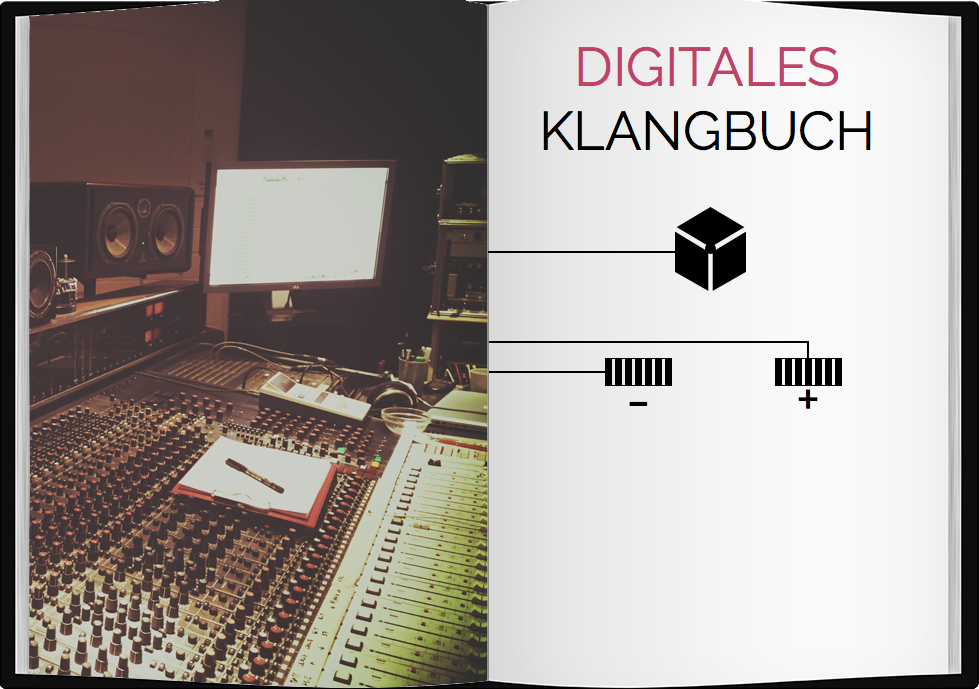
\includegraphics[width=1.0\textwidth]{grafiken/bsplinien.png}
\caption{Beispiel-Inhalt eines digitalen Klangbuchs: Auf der linken Seite ist ein Bild abgedruckt. Berührungsempfindliche Elemente auf der rechten Seite wurden mit einer speziellen Tinte gedruckt und sind mit einer schwarzen Linie mit dem Buchrücken verbunden. Bei Berührung lösen sie eine Funktion aus. Wird der Würfel (unterhalb der Überschrift) berührt, startet der \gls{song}. Bei wiederholter Berührung wird der \gls{song} gestoppt. Die Lautstärke kann ebenfalls beeinflusst werden (Berührung der Felder über das Plus- und Minuszeichen)\\Foto: Sahrah El ghammaz}
\label{fig:klangbuch1}
\end{figure}

Durch das Hören der Musik, das Betrachten der Bilder, Grafiken und Texte und durch das Berühren / Interagieren mit dem Buch werden mehrere Sinne angesprochen und damit ein besonderes Erlebnis geschaffen. Durch das Klangbuch kann der Fan eine Bindung zu der Musik und dem Künstler aufbauen. Dadurch, dass der Fan ein Buch in den Händen hält, mit dem er interaktiv agieren kann, nimmt er sich mehr Zeit für die Musik. Ein Musikalbum wird mit dem digitalen Klangbuch zu einem Gesamterlebnis aufgewertet.



\section{Das Praxisprojekt}
Die Entwicklung des digitalen Klangbuchs ist ein Projekt, das aus vielen Teilprojekten besteht. Eines dieser Teilprojekte ist die Beantwortung der Frage: Was sind geeignete technologische Ansätze um ein digitales Klangbuch zu entwickeln?\\ 
Ziel des Praxisprojekts war es diese Frage zu beantworten. Dazu wurden verschiedene Technologien recherchiert, teilweise getestet und bewertet. Diese lassen sich grob in folgende Kategorien unterteilen: Digitales und Elektronisches Papier, Leitende Tinte, Gedruckte Elektronik und klassische elektronische Bauteile.\\
Anschließend wurden, auf Basis der Technologien, grobe Realisierungsansätze eines digitalen Klangbuchs entwickelt. 
Die Arbeit konnte mit dem Ergebnis abgeschlossen werden, dass es viele Technologien gibt, mit denen ein digitale Klangbuch entwickelt werden kann. Die recherchierten Technologien können einzeln, aber auch kombiniert eingesetzt werden.\\
Im Ausblick des Praxisprojekt wurden folgende, weitere Teilprojekte zum Gesamtprojekt "Digitales Klangbuch" vorgeschlagen:

\begin{itemize}
\item Recherche Komponenten: Weiter Komponenten, wie z. B. ein Mikrocontroller, müssen recherchiert und getestet werden.
\item Programmierung: Für die Steuerung des Buches ist die Programmierung des Mikrocontrollers notwendig.
\item Funktionaler Prototyp: Ein funktionierender Prototyp, der eine ausgewählte Technologie, die Komponenten und die Programmierung enthält, wird entwickelt.
\item Funktionsleitfaden: Erarbeitung und Gestaltung eines Leitfadens, der die Funktionen des digitalen Klang- Buchs erläutert und veranschaulicht.
\item Gestaltung: Nach Auswahl eines Realisierungsansatzes und in Kooperation eines Künstlers / einer Band wird der Inhalt des Buches passend zu den Audiodateien gestaltet.
\item Gestalteter, funktionaler Prototyp und Auswertung: Ein minimalistischer, jedoch gestalteter und funktionaler Prototyp wird entwickelt und getestet.
\item Finanzierungsmöglichkeiten: Es werden verschiedene Finanzierungsmöglichkeiten zur Entwicklung des Buches untersucht und ausgewertet.
\item Crowdfunding: Es wird eine \gls{crowdfunding}-Kampagne zur Finanzierung der Buchentwicklung entwickelt und gestartet.
\item Anwendungsfälle: Es werden weitere Möglichkeiten / Anwendungsfälle zum Einsatz des Buches ermittelt.
\end{itemize}




%{\centering\textcolor{m_pink}{\textit{"Nach dem Einkauf trugen wir die Platten (...) nach Hause, legten sie andächtig auf den Plattenteller (...) und beschäftigten uns tagelang mit den Alben."}}\\\hfill\begin{tiny}{Klaus Warstat \cite{K01}}\end{tiny}}\\



%%%%%%%%%%%%%%%%%%%%%%%%%%%%%%%%%%%%%%%%%%%%%%%%%%%%%%

\section{Entscheidung Bachelorthema \& Problemstellung}\label{einleitung_problem}
Die Wahl auf eines der Teilprojekte zur Fortführung des Gesamtprojekts "Digitales Klangbuch" wurde aufgrund folgender Kriterien getroffen:\\

1. Das Thema sollte innerhalb des zeitlichen Rahmens der Bachelorarbeit realisierbar sein.\\
2. Die Kosten sollten möglichst gering sein.\\
3. Die Bachelorarbeit soll das Gesamtprojekt "Digitales Klangbuch" voran treiben.\\
4. Die Abhängigkeit von Dritten soll möglichst gering sein.\\

Ein Proof of Concept der Technologien und der Komponenten konnte aufgrund der Kosten und der Verfügbarkeit\footnote{Verfügbarkeit: Im Sinne von Zugriff, Zugänglichkeit für Nicht-Fachkräfte} der Technologien nicht in Betracht gezogen werden. Die Technologie "Leitende Tinte" wurde jedoch bereits im Rahmen einer Vorstudie erfolgreich erprobt. Die übrigen Teilprojekte sind teilweise voneinander abhängig, so dass diese ebenfalls nicht für die Bachelorarbeit geeignet sind.\\

Die Wahl fiel daher auf die Entwicklung eines Leitfadens um die Möglichkeiten und Grenzen des digitalen Klangbuchs zu erläutern und zu veranschaulichen:\\
Das digitale Klangbuch und dessen Möglichkeiten sind für außenstehende Personen nicht einfach zu verstehen. Zum Einen, weil das digitale Klangbuch eine abstrakte und neue Idee ist, die man (noch) nicht berühren oder ausprobieren kann. Aber auch, weil die Technologien, die zum Einsatz kommen könnten, für viele Menschen neu und fremd sind. Ein Künstler / Musiker, der Inhalte für das digitale Klangbuch kreieren möchte, weiß schlechtenfalls nicht, welche Möglichkeiten zur Darstellung und Interaktion seiner Inhalte das Buch bietet. Da das digitale Klangbuch weit über ein normales Album und ein \gls{artwork} hinaus geht, sind dem Künstler / Musiker weder die Vielfalt der Möglichkeiten, noch die Grenzen des Buches bekannt.




%%%%%%%%%%%%%%%%%%%%%%%%%%%%%%%%%%%%%%%%%%%%%%%%%%%%%%
\section{{Zielsetzung der Bachelorarbeit}}\label{einleitung_ziel}
Ein Leitfaden, der die Funktionen des digitalen Klangbuchs erläutert und veranschaulicht, würde dem Interessierten die visuellen, auditiven und haptischen Möglichkeiten zur interaktiven Darstellung und Integration von Text, Grafik, Bild und Audio des digitalen Klangbuchs veranschaulichen und ihn idealerweise inspirieren. Hier ein Beispiel:\\

Eine mögliche Funktion des digitalen Klangbuchs wäre die interaktive Darstellung einer Mehrspuraufnahme. Die einzelnen Spuren eines \gls{song}s werden in das Buch integriert und können vom Hörer stumm geschaltet, oder die Lautstärke der einzelnen Spuren angepasst werden. Der Hörer kann so interaktiv den \gls{song} nach seinen Wünschen verändern und seine eigenen \gls{remix}e erstellen.\\

Die Forschungsfrage der Bachelorarbeit lautet: Wie lassen sich die Möglichkeiten und Grenzen des digitalen Klangbuchs Musikern und Künstlern vermitteln und wie lässt sich ein nichtfunktionaler, real aussehender Prototyp des digitale Klangbuch entwickeln?\\

Neben dem Hauptziel, Musikern und Künstlern die Möglichkeiten und Grenzen des Klangbuchs aufzuzeigen, können zwei weitere Ziele mit dem Vorhaben erreicht werden. Das digitale Klangbuch ist bislang nur ein Konzept. Mit einem Leitfaden, der das digitale Klangbuch und seine Möglichkeiten und Funktionen präsentiert, kann eruiert werden, inwieweit Interesse an einem solchen Konzept besteht. Darüber hinaus ist der Leitfaden ein gutes Hilfsmittel um mit Musikern und Künstlern in den Dialog zu treten.




\section{{Zielgruppe}}\label{einleitung_zielgruppe}
Das primäre Nutzungsszenario des digitalen Klangbuchs liegt im Bereich Musik / Kunst / \gls{artwork}. Die Zielgruppe, die das Buch mit Inhalten (Musik, Kunst, Texte, etc.) füllt, sind Musiker / Künstler. Musiker, die ein Musikalbum mit dem digitalen Klangbuch abbilden möchten und Künstler, die Informationen, Fotografien, Bilder und künstlerische Arbeiten, passend zur Musik des Albums kreieren möchten. Arbeiten Musiker und Künstler zusammen, kann ein Gesamtwerk aus Musik, \gls{artwork} und Interaktion geschaffen werden. An diese Zielgruppe richtet sich der Leitfaden. Die Zielgruppe wird im weiteren Verlauf der Arbeit "KlangKünstler" genannt. Ist eine Differenzierung notwendig, kommen die Begriffe "Musiker" und "Künstler" zum Einsatz. Der Nutzer, der am Ende das fertige Buch in den Händen hält, wird als Hörer oder Fan bezeichnet.\\








%%%%%%%%%%%%%%%%%%%%%%%%%%%%%%%%%%%%%%%%%%%%%%%%%%%%%%
\section{{Vorgehen}}\label{einleitung_vorgehen}

Die Bachelorarbeit ist im Bereich Musik, Kunst und (Web-)Technik platziert. Es werden daher fachspezifische Begriffe verwendet, die im angehängten Glossar erläutert werden.\\

Die Bachelorarbeit lässt sich in folgende Hauptbereiche festlegen, die in den zugehörigen Kapiteln näher erläutert und unterteilt werden:

\begin{itemize}
\item Recherche möglicher Arten von Leitfäden
\item Entscheidung für eine Leitfadenart
\item Ideen und Entwicklung möglicher Funktionen des digitalen Klangbuchs
\item Konzeption eines Leitfadens
\item Umsetzung des Leitfadens
\item Der Leitfaden
\item Fazit
\item Ausblick
\end{itemize}




%%%%%%%%%%%%%%%%%%%%%%%%%%%%%%%%%%%%%%%%%%%%%%%%%%%%%%
\section{{Motivation}}\label{einleitung_motivation}
Die Bachelorarbeit setzt, wie bereits in der Einleitung erklärt, das Praxisprojekt fort. Die Motivation zur Erarbeitung des digitalen Klangbuches in Bezug auf die Bachelorarbeit ist ähnlich der des Praxisprojekts:

"Bei der Themenfindung habe ich versucht die Themen zu kombinieren, die mir wichtig sind - Musik, Kunst, Kreativität und Entwicklung - und diese in einen Bezug zur Medieninformatik zu stellen. Vor allem zur Musik habe ich eine besondere und tiefe Verbindung. Das Thema Musik war schon Bestandteil in verschiedenen vorangegangenen Projekten.\footnote{„Live in Concert“, MCI/MMA Projekt bei Prof. Dr. Hartmann \url{http://bit.ly/XxN0N3}}‘\footnote{„Dynamische Soundanalyse“, WPF Generative Gestaltung bei Prof. Noss \url{http://bit.ly/1RYEc2J}}\\

Wie bereits in der Einleitung erläutert, verlieren Audiowerke durch die einfache Möglichkeit an Vervielfältigung an Wert. Musik ist nicht mehr ein reines Genusswerk, sondern wird konsumiert und weniger wertgeschätzt. Der Hörer, inklusive meiner Person, nimmt sich weniger Zeit und Ruhe um ein Audiowerk zu genießen und mehr über den Künstler und sein Werk zu erfahren. Musik wird nicht mehr als Kunst wertgeschätzt, sondern verkommt zu einem Grundrauschen. Das möchte ich mit diesem Projekt ändern."\cite{pp}\\

Dieses Ziel verfolge ich auch mit dieser Arbeit.\\

Das Praxisprojekt bestand zu einem großen Teil aus der Recherche geeigneter Technologien um ein digitales Klangbuch entwickeln zu können. Die Bachelorarbeit dagegen soll weniger aus Recherche bestehen, sondern durch praktische Auseinandersetzung mit unterschiedlichen Aspekten des Klangbuchs das Gesamtprojekt voran treiben und für Künstler und Musiker greifbar machen.



%\item Geschichte der Tonträger und des \gls{artwork}s
%\item Ideen und Ansätze aus der Buchkunst







 







